\documentclass[11pt]{amsart}
\usepackage[margin=1.2in]{geometry}                % See geometry.pdf to learn the layout options. There are lots.
\geometry{letterpaper}                   % ... or a4paper or a5paper or ... 
%\geometry{landscape}                % Activate for for rotated page geometry
%\usepackage[parfill]{parskip}    % Activate to begin paragraphs with an empty line rather than an indent
\usepackage{graphicx}
\usepackage{amssymb}
\usepackage{epstopdf}
\usepackage[colorlinks=true, pdfstartview=FitV, linkcolor=blue, citecolor=blue, urlcolor=blue]{hyperref}
 \usepackage{tikz}
\usepackage[listings]{tcolorbox}
\usepackage{caption}
\usepackage{subcaption}
\usepackage{mathrsfs}
\usepackage{enumitem}
\usepackage{verbatim}
\usepackage{animate}
\usepackage[smalltableaux]{ytableau}
\usepackage[nameinlink]{cleveref}
%\usepackage[symbol]{footmisc}
\DeclareGraphicsRule{.tif}{png}{.png}{`convert #1 `dirname #1`/`basename #1 .tif`.png}
\newcommand\userinput[1]{{\bf #1}}

\crefname{defn}{definition}{definitions}
\Crefname{def}{Definition}{Definitions}
\crefname{thm}{theorem}{theorems}
\Crefname{thm}{Theorem}{Theorems}

%=========== colors ====
\usepackage{color}
\newcommand{\cc}{\color{cyan}}
\newcommand{\cb}{\color{blue}}
\newcommand{\cm}{\color{magenta}}

%=========== fraktur letters ====

\newcommand{\m}{{\mathfrak M}}
\newcommand{\fp}{{\mathfrak p}}

%========== bold letters =========

\newcommand{\C}{{\mathbb C}}
\newcommand{\F}{{\mathbb F}}
\newcommand{\N}{{\mathbb N}}
\newcommand{\R}{{\mathbb R}}
\newcommand{\Q}{{\mathbb Q}}
\newcommand{\Z}{{\mathbb Z}}

\newcommand{\ba}{{\mathbf a}}
\newcommand{\bb}{{\mathbf b}}
\newcommand{\bc}{{\mathbf c}}
\newcommand{\be}{{\mathbf e}}
\newcommand{\bp}{{\mathbf p}}
\newcommand{\bx}{{\mathbf x}}
\newcommand{\bv}{{\mathbf v}}

%========== mathcal letters =========

\newcommand{\M}{{\mathcal M}}
\renewcommand{\O}{{\mathcal O}}
\renewcommand{\P}{{\mathcal P}}
\newcommand{\A}{{\mathcal A}}
\newcommand{\cH}{{\mathcal H}}
\newcommand{\B}{{\mathcal B}}
\newcommand{\K}{{\mathcal K}}
\newcommand{\T}{{\mathcal T}}
\newcommand{\Pf}{\rm{Pfaff}}
\newcommand{\cP}{{\mathcal P}}
\newcommand{\cS}{{\mathcal S}}
\newcommand{\cF}{{\mathcal F}}

%=========== operators ==============

\def\Ass{\operatorname{Ass}}
\def\Cat{\operatorname{Cat}}
\def\Hom{\operatorname{Hom}}
\def\depth{\operatorname{depth}}
\def\Ext{\operatorname{Ext}}
\def\Fl{\operatorname{Fl}}
\def\Jac{\operatorname{Jac}}
\def\supp{\operatorname{supp}}
\def\conv{\operatorname{conv}}
\def\Im{\operatorname{Im}}
\def\Jac{\operatorname{Jac}}
\def\height{\operatorname{ht}}
\def\gin{\operatorname{gin}}
\def\codim{\operatorname{codim}}
\def\bht{\operatorname{bight}}
\def\Span{\operatorname{Span}}
\def\MSpec{\operatorname{MaxSpec}}
\def\rank{\operatorname{rank}}
\def\Ann{\operatorname{Ann}}
\def\im{\operatorname{im}}
\def\lcm{\operatorname{lcm}}
\def\lra{\longrightarrow}
\def\ord{\operatorname{ord}}
\def\reg{\operatorname{reg}}
\def\sat{{\rm sat}}
\def\sdef{\operatorname{sdef}}
\def\sgen{\operatorname{sgen}}
\def\sdl{\operatorname{sdl}}
\def\sl{\operatorname{sl}}
\def\lc{\operatorname{lc}}
\def\htt{\operatorname{ht}}
\def\edim{\operatorname{edim}}
\def\bm{\mathbf{m}}
\def\n{\mathfrak{n}}
\def\Max{\operatorname{Max}}
\def\ha{\widehat{\alpha}}
\def\ov{\overline}
\def\vol{\operatorname{vol}}
\def\init{{\rm in}}
\def\str{\operatorname{str}}
\def\sym{S}
\def\l{\lambda}
\def\Seg{\operatorname{Seg}}
\newcommand{\dSdw}{\Delta}
\newcommand{\uSdw}{\rotatebox[origin=c]{180}{$\Delta$}}
\def\lex{\operatorname{lex}}
\newcommand{\di}{\diamond}
\renewcommand*{\thempfootnote}{\fnsymbol{mpfootnote}}


%========= theorems =============

\theoremstyle{plain} %% This is the default, anyway
\newtheorem{thm}{Theorem}[section]
\newtheorem{thmdef}[thm]{TheoremDefinition}
\newtheorem{introthm}{Theorem}
\newtheorem{introcor}[introthm]{Corollary}
\newtheorem*{introthm*}{Theorem}
\newtheorem{question}{Question}
\newtheorem{cor}[thm]{Corollary}
\newtheorem{lem}[thm]{Lemma}
\newtheorem{prop}[thm]{Proposition}
\newtheorem{probl}[thm]{Problem}
\newtheorem{oprobl}{Open Problem}
\newtheorem*{oprobl*}{Open Problem}


\newtheorem{conj}[thm]{Conjecture}
\newtheorem{quest}[thm]{Question}

\theoremstyle{definition}
\newtheorem{defn}[thm]{Definition}
\newtheorem{chunk}[thm]{}
\newtheorem{ex}[thm]{Example}
\newtheorem{exer}[thm]{Exercise}
\newtheorem{alg}[thm]{Algorithm}

\theoremstyle{remark}
\newtheorem{rem}[equation]{Remark}
\newtheorem{notation}[thm]{Notation}
\newtheorem{terminology}[equation]{Terminology}

\numberwithin{equation}{section}  %% equation numbering


\title{Macaulay Rings and Macaulay Posets}
\author{Nikola Kuzmanovski and Alexandra Seceleanu}
%\date{}                                           % Activate to display a given date or no date

\begin{document}
\maketitle

\begin{abstract}
%\vspace{-2em}
This document describes a research project for the Polymath REU program in summer of 2024. Please do not share it with anyone who is not part of the program.
\end{abstract}

\graphicspath{{pictures}}

\subsection*{How to read this document.}
 You might want to first skim this document without dwelling too much on the technicalities. The questions that will be discussed in this project are marked as ``open problems'' and are located in  \cref{s:3}. Read them carefully and consider whether you might be interested in exploring these problems further. Make sure to read the definitions and examples of concepts appearing in these problems. Section \ref{s:background} is designed to help you with this. Paragraphs marked as exercises can be ignored in a first scan.  
 
 I am not assuming any pre-requisite knowledge, however having had a course in abstract algebra will be very helpful. It will also help if you know some linear algebra, combinatorics, or programming, but none of these are required. In the first weeks of the program we will work through understanding the background in \cref{s:background} and \cref{s: 2}. In fact, a thorough understanding of the mathematics introduced in this document  can  in itself be your objective for the duration of the program. If you decide to be part of this project, then it is strongly recommended to start by spending some time on the exercises early on. The students involved in this project will collaborate on writing solutions to many if not all of the exercises. If you are having a hard time with a concept or exercise, ask for a hint or help in the Discord project channel. %Ask for a solution only after spending enough time trying to solve the problem.  
 
 There are several open questions listed in \cref{s:3} of this document. At the end of the second week of the program you will pick {\em one} problem in that project to work on. In the following weeks students will get together with others working on the same sub-project to exchange ideas. Our main goal during this program is to compute {\em a lot of examples} and come up with conjectured answers to some of the open problems.  If we can prove some of our conjectures all the better! Most likely the answer to many of the open questions is no, so you should probably focus on coming up with counterexamples before trying to prove anything. It might be hard to start  on the open problems without working out the exercises first. Similarly, it might be hard to start working on the open problems on your own, without guidance. Feel free to ask the mentors for first directions. 

Participants in this project will benefit from exploration using computer algebra systems. For this reason, we will learn to use {\em Macaulay 2}. We will prepare a quick tutorial to get you started, which will take place in the second week of the program (see also the Macaula2 introductory document),  but there are also many online resources to help you get familiar with this software on its webpage  \cite{M2}. You are also welcome to ask the mentors about it. 

\section{Background}
\label{s:background}

In this project we will encounter mathematical concepts coming from commutative algebra -- mainly polynomials and ideals -- and combinatorics -- partially ordered sets (or posets). The purpose of this section is to give a brief introduction to some commutative algebra and combinatorics notions. You will need to gain some familiarity with these concepts to understand the problems we will be working on. 

\subsection{Polynomials in several variables}

Without further ado, we introduce the main objects of study in this text. In these notes the letter $K$ denotes a field, for example $\Q$ (the rational numbers), $\R$ (the real numbers), $\C$ (the complex numbers) or $\F_p$ (the integers modulo $p$, where $p$ is a prime integer). If $K$ contains $\Q$ we say $K$ has {\em characteristic zero} (for example, $\Q, \R, \C$ are fields of characteristic zero), while if $K$ contains $\F_p$ we say $K$ has {\em characteristic p} (for example $\F_p$ has characteristic $p$). Equivalently, $p=0$ in a field of characteristic $p$, but no positive integer is zero in a field of characteristic $0$.

The natural numbers, including 0, will be denoted $\N$.

Let us now review polynomials in one variable, which should be familiar to you. Let $x$ be a variable. A polynomial in the variable $x$ with coefficient in the field $K$ is an expression 
\[
p(x)=a_0+a_1x+a_2x^2+ \cdots + a_nx^n \text{ where }n\geq 0 \text{ and } a_0, a_1, \ldots, a_n \text{ are elements of }K.
\]
For example, $3+10x-x^2+5x^5$ is a polynomial.
We denote the set of all such polynomials by $K[x]$. This set comes equipped with operations of  adding and multiplying polynomials. %Whenever a set has such operations, we say it is a  ring. 

\smallskip

Next we consider polynomials in several variables, for now, in the variables x,y,z. 

\begin{ex}\label{ex: x y z}
The expression $2x^3+xy+7yz+11z-100$ is a polynomial in variables $x,y,z$. 
We can add and multiply such polynomials according to the usual rules
 \begin{eqnarray*}
 (2x^3+xy+7yz+11z-100) +(z^3-xy +xz+6yz)=2x^3+z^3+xz+13yz+11z-100\\
 (2x^3+xy+7yz+11z-100)(z+1)=2x^3z+xyz+7yz^2+11z^2+2x^3+xy+7yz+z-10.
\end{eqnarray*}
We denote by $\R[x,y,z]$ is the set of polynomials in the variables $x,y,z$ with real coefficients.
\end{ex}

A particularly simple kind of polynomials are {\bf monomials}. These are polynomials with a single term and no coefficient (or rather they have a coefficient equal to 1). The monomials which appear in the polynomials in \Cref{ex: x y z} are: $x^3,z^3, xy, xz,yz,z, 1, x^3z, xyz, yz^2, z^2$. 

Monomials have {\bf exponent vectors}, for example, $xyz=x^1y^1z^1$ has exponent vector $(1,1,1)$ and $x^3z=x^3y^0z$ has exponent vector $(3,0,1)$. When considering exponent vectors one has to be aware in how many variables we are working. For example, the exponent vector of $xy$ is $(1,1)$ if we think of it as a polynomial $K[x,y]$, that is, in two variables $x$ and $y$, but  the exponent vector of $xy$ is $(1,1,0)$ if we think of it as a polynomial $K[x,y,z]$. We can plot these exponent vectors as points in 2-space or 3-space, depending on the number of variables. or as boxes in a ``box diagram" as shown below.

%\begin{ex}
\begin{center}
	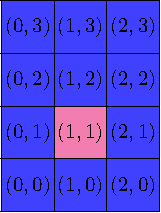
\includegraphics[height=3.5cm]{Pictures/2D_3_4_<1,1>.pdf}
	\qquad 
	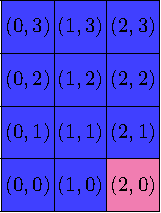
\includegraphics[height=3.5cm]{Pictures/2D_3_4_<2,0>.pdf}
	\qquad 
	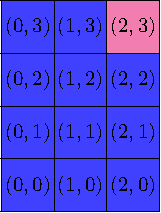
\includegraphics[height=3.5cm]{Pictures/2D_3_4_<2,3>.pdf}
\end{center}
%\end{ex}

To go beyond two or three variables, we now consider several variables $x_1, \ldots, x_n$ and form polynomials using them. We can now make the notions described above more rigorous.
\tcbset{colback=white}
\begin{tcolorbox}
\begin{defn} A {\bf monomial} in the set of  variables $x_1, \ldots, x_n$  is  a product of powers of the variables of the form $x_1^{a_1}x_2^{a_2} \cdots x_n^{a_n}$, with $a_i\in \N$. For example $x_1^2x_2x_4^5$ is a monomial. 
We often denote monomials by using shorthand (vector) notation
\[
\bx^\ba =x_1^{a_1}x_2^{a_2} \cdots x_n^{a_n}.
\]
In this way, each monomial $\bx^\ba$ corresponds to a vector $\ba=(a_1,\ldots, a_n)\in \N^n$. 
%A monomial $\bx^\ba$ is square-free if  each entry of $\ba$ is either 0 or 1.
\end{defn}
\end{tcolorbox}

\begin{tcolorbox}[reset]
\begin{exer}
Explain why $1$ is always a monomial but $0$ is not.
\end{exer}
\end{tcolorbox}


\begin{tcolorbox}
\begin{defn} A {\bf polynomial} in the set of  variables $x_1, \ldots, x_n$ with coefficients in a field $K$ is a $K$-linear combination of monomials, that is an expression of the form
\[
f(\bx)= \sum _{\ba\in E} c_\ba x_1^{a_1}x_2^{a_2} \cdots x_n^{a_n},
\]
where $E$ is a {\em finite} subset of  $\N^d$, which represents the set of exponents of monomials in our polynomial, and for each $\ba=(a_1,\ldots, a_n)\in E$, $c_\ba$ is an element of the field $K$. %Note that we use the bold letter $\bx$ to denote the tuple of variables $\bx=x_1, \ldots, x_n$.
\end{defn}
\end{tcolorbox}

\begin{ex}
The expression $2x_1^3+x_1x_2+7x_2x_3-100$ is a polynomial in variables $x_1, x_2, x_3$ with coefficients in $\R$. 
\end{ex}



\begin{tcolorbox}
\begin{defn} For $K$ a field, the set  
\[
K[x_1,\ldots , x_n]=\left  \{p(\bx) : p(\bx) \text{ a polynomial in variables }x_1,\ldots x_n \text{ with coefficients in }K \right \}
\]
is called the {\bf polynomial ring} on $n$ variables with coefficients in $K$. 
\end{defn}
\end{tcolorbox}
We call this set a ring because it is endowed with addition and multiplication and these operations satisfy certain properties, like distributivity of multiplication over addition, that you are  familiar with. Incidentally, there are many other rings out there. For example, the set $\Z$ of integers is a ring and so are the sets $\Q, \R, \C, \F_p$ described above.

The polynomial ring is a {\bf commutative ring} since multiplication of polynomials is commutative, that is, it obeys the rule that $f(\bx)g(\bx)=g(\bx)f(\bx)$ for any polynomials $f(\bx),g(\bx)$. {\bf Commutative algebra} is the study of commutative rings. A nice introduction to commutative algebra at the undergraduate level, focusing primarily on polynomials, is \cite{CLO}.


\subsection{Ideals of the polynomial ring}
\begin{notation}
Throughout these notes we denote $R=K[x_1,\ldots, x_n]$. \Cref{def:ideal} and  \Cref{def:gens} can be formulated for arbitrary rings, but we don't need them in that generality.
\end{notation}

\begin{tcolorbox}
\begin{defn}\label{def:ideal}
An {\bf ideal} of a commutative ring $R$ is a nonempty subset $I\subseteq R$ that satisfies:
\begin{itemize}
\item (closure under $+$) if $f,g \in I$ then $f+g\in I$
%\item (zero element) the zero polynomial is an element of $I$
\item (closure under $\cdot$) if $r\in R$ and $f\in I$ then $rf\in I$. 
\end{itemize}
\end{defn}
\end{tcolorbox}
In particular the second property gives that if $f\in I$ then its negative $-f=(-1)f\in I$ and also that the zero polynomial $0=0\cdot f$ is in $I$. 
Notice that closure under $+$ applies to two elements of $I$ while closure under $\cdot$ applies to an element of $R$ and  an element of $I$.

\begin{tcolorbox}[reset]
\begin{exer}\label{exercise}
Prove that the set below is an ideal in $K[x,y]$:
\[
I=\{f\in K[x,y]: f= x^2g+ y^3h \text{ for some } g,h\in K[x,y]\}.
\]
\end{exer}
\end{tcolorbox}


\begin{tcolorbox}[reset]
\begin{exer}\label{ex: maximal ideal}
Show that the set $\m$ of all polynomials in $R=K[x_1,\ldots, x_d]$ with  constant term equal to 0 is an ideal of $R$. It is called the {\em homogeneous maximal ideal}.
\end{exer}
\end{tcolorbox}

\begin{tcolorbox}
\begin{defn} 
\label{def:gens}
The {\bf ideal generated by} elements $g_1, \ldots, g_t$ of $R$, denoted $(g_1, \ldots, g_t)$, is the set of finite $R$-linear combinations of $g_1, \ldots, g_t$, formally
\[
(g_1, \ldots, g_t)=\{ r_1g_1+r_2g_2+\cdots + r_tg_t \mid r_i\in R\}.
\]
For example, we can write the set $I$ in \Cref{exercise} as $I=(x^2,y^3)$.
\end{defn}
\end{tcolorbox}
It is important to note that in the definition above $r_1, \ldots, r_t$ are elements of $R$ (polynomials) not elements of $K$ (scalars). %We say that $g_1, \ldots, g_t$ minimally generate an ideal $I$ or are {\bf minimal generators} of $I$ if $I=(g_1, \ldots, g_t)$ and no proper subset of $g_1, \ldots, g_t$ generates $I$.

\begin{tcolorbox}[reset]
\begin{exer}
Show that the homogeneous maximal ideal from \Cref{ex: maximal ideal} is generated by the variables $x_1, \ldots, x_n$, in symbols  $\m=(x_1,\ldots, x_n)$.
\end{exer}
\end{tcolorbox}

\begin{tcolorbox}
\begin{defn}
A very useful property of polynomial rings is the existence of a {\em degree function} $\deg:R\to\N$.
The {\bf degree} of the monomial $\bx^\ba =x_1^{a_1}x_2^{a_2} \cdots x_n^{a_n}$, is 
\[
\deg(x_1^{a_1}x_2^{a_2} \cdots x_n^{a_n} )=a_1+a_2+\cdots+a_n.
\]
A polynomial $f$ is {\bf homogeneous} if it can be written as a $K$-linear combination of monomials of the same degree. In this case, the degree of $f$ is defined to be the degree of any of the monomials of $f$.
\end{defn}
\end{tcolorbox}


\begin{ex}
The polynomial $f=2x^2+xy^3$ is not homogeneous since $\deg(x^2)=2\neq 4=\deg(xy^3)$. The polynomial $g=2x^2-xy+6y^2$ is homogeneous of degree $\deg (g)=2$.
\end{ex}

%One can extend the notion of degree from polynomials to ideals. 
%\begin{defn}
%The {\em initial degree} of a ideal $I$ is $\alpha(I)=\min\{\deg(f) \mid \bx^\ba\in I\setminus\{0\}\}$.
%\end{defn}
%
%\begin{ex}
%The initial degree for the ideal  $I = (2x^2-xy+6y^2, xy^3+7x^2z^2)$ is $\alpha (I)=2$.
%\end{ex}





\begin{tcolorbox}
\begin{defn}
An ideal that can be generated by homogeneous polynomials is called a {\bf homogeneous ideal}.
\end{defn}
\end{tcolorbox}

\begin{tcolorbox}
\begin{defn} A {\bf monomial ideal} in $R$ is an ideal of $R$ that can be generated by monomials. Monomial ideals are homogeneous.
\end{defn}
\end{tcolorbox}

\begin{ex} Consider $R = K[x,y]$. The ideal $I = (x^2, y^3)$ is a monomial ideal, hence homogeneous. Note that I contains the polynomial $x^2 - y^3$, so monomial ideals contain more than just monomials. 
The ideal $J = (y^3-x^2, x^2)$ is also a monomial ideal because  $J=I$. In the picture below we plot in pink all the monomials which are in the ideal $I$ and in blue all the monomials which are {\em not} in the ideal $I$.
\begin{center}
	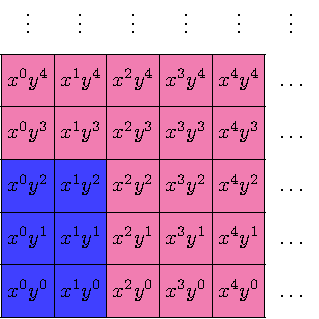
\includegraphics[height=5cm]{Pictures/<x^2,y^3>.pdf}
\end{center}
\end{ex}

\begin{tcolorbox}[reset]
\begin{exer}
Show that a monomial $\bm$ belongs to the ideal generated by monomials $\bm_1,\ldots, \bm_t$ if and only if  $\bm$ is divisible by $\bm_i$ for some $1\leq i\leq t$.
\end{exer}
\end{tcolorbox}

\begin{tcolorbox}[reset]
\begin{exer}\label{ex:monomialmingens}
Show that a monomial ideal has a unique set of minimal generators which are monomials. We call a set of generators {\em minimal} if no proper subset generates the same ideal.
\end{exer}
\end{tcolorbox}

\subsection{Quotient rings}

If $I$ is an ideal of a ring $R$ and $r$ is an element of $R$ we call the set
\[
r+I=\{ r+a : a\in I\}
\]
the {\bf coset} of $r$ modulo $I$.
Caution: two seemingly different cosets can in fact be equal .
\begin{tcolorbox}[reset]
\begin{exer}
Show that $r_1+I=r_2+I$ if and only if $r_1-r_2\in I$.
\end{exer}
\end{tcolorbox}
\begin{tcolorbox}
\begin{defn} The  {\bf quotient ring} $R/I$ of a ring $R$ by an ideal $I$ of $R$ is  the set 
\[
R/I=\{r+I : r\in R\}
\]
with operations described  by
\begin{itemize}
\item $(r_1+I)+(r_2+I)=(r_1+r_2)+I$ 
\item $(r_1+I)\cdot (r_2+I)=(r_1r_2)+I$
\end{itemize}
The element $0+I$ is called the zero element of $S$.

If $I$ is a homogeneous ideal we say that $R/I$ is a homogeneous or graded ring.
\end{defn}
\end{tcolorbox}

\begin{ex}
For the ring of integers $\Z$ the ideals are the sets $(n)=\{nk \mid k\in \Z\}$ and the corresponding quotient rings $\Z/(n)$ are the rings of integers modulo $n$.
\end{ex}

\begin{tcolorbox}
\begin{defn}\label{Monomials_and_Monomial_Ideals_Definition}
 Let $R=K[x_1,\dots, x_n]$ and $S=R/I$, where $I$ is a homogeneous ideal of $R$,  $I\neq R$. 
A {\bf monomial of $S$} is a \underline{nonzero} element of $S$ of the form $\bx^\ba + I$, where $\ba \in \N^d$.
A {\bf monomial ideal} of $S$ is an ideal of $S$  generated by monomials.
	\end{defn}
	\end{tcolorbox}

\begin{ex}
Let $S=K[x,y]/(x^2,y^2)$ and let $I=(x^2,y^2)$. This ring has four monomials: $1+I, x+I, y+I$, and $xy+I$. The element $x^2+I$ of $S$ is {\em not} a monomial because it is equal to $0+I$, that is, it is zero in $S$.
\end{ex}
%\begin{tcolorbox}[reset]
%\begin{exer}
%Show that if $R$ is the polynomial ring and $m$ is as in \cref{}, then $R/\m\cong K$. 
%\end{exer}
%\end{tcolorbox}

\subsection{Partially ordered sets from monomials}
\phantom{a}

In many sets we have a way to compare any two elements. If that is the case we say that we have a {\em total order} on the set. For example, a familiar example of a set with a total order is the real numbers with the usual order where, e.g. $3 \leq \pi$. 

However, in others sets it could be that some pairs of elements are comparable but others are not comparable. In this context we say that we have a {\em partial order}. For example, if our set is the natural numbers we can compare two elements $a$ and $b$ by saying that $a\leq b$ means $a$ divides $b$. In this case $4$ and $8$ are {\em comparable} since $4\mid 8$ but $4$ and $11$ are {\em incomparable}. 

\begin{tcolorbox}
\begin{defn}\label{def: partial order}
A {\bf partially ordered set (poset)} is a set $\P$ which has an order relation on it, that is, a binary relation denoted $\leq$ which satisfies
\begin{itemize}
\item $a\leq a$ for all $a\in \P$
\item if for some $a,b\in \P$ we have $a\leq b$ and $b\leq a$, then $a=b$
\item if for some $a,b,c \in \P$ we have $a\leq b$ and $b\leq c$, then $a\leq c$.
\end{itemize}
\end{defn}
\end{tcolorbox}

\begin{defn}
A {\bf total order}  on a set $\P$ is a binary relation that satisfies the three conditions in \Cref{def: partial order} but for which every pair of elements of $\P$ is comparable.
\end{defn}

As per usual, we write $a<b$ to denote that $a\leq b$ and $a\neq b$.

 A poset $\P$ is sometimes pictured as a graph, called the {\bf Hasse graph} of $\P$. In this graph, an edge connects two elements $a,b\in \P$ so that $b$ {\bf covers} $a$, that is, $a<b$ and there is no $c$ that satisfies $a<c<b$. (In the example of divisibility on $\N$, $8$ covers $4$.)  In the picture $a$ will be placed lower than $b$. All  other inequalities can be inferred from this information.




\begin{ex}
A {\em path poset of length $d$} is a poset on $d$ vertices $0,\ldots, d$ which is totally ordered by the ordering of $0,\ldots, d$ as real numbers. The Hasse graph for $d=3$ is
\begin{center}

\includegraphics[height=2cm]{Pictures/Spider_legs_1_length_2.pdf}
\end{center}
\end{ex}

\begin{ex}
A {\em basic star poset with $n$ legs} is a poset on $n+1$ vertices having a distinguished vertex $\ell$ such that $\ell\leq a$ for every vertex $a$ of the poset and there are no other comparisons. The Hasse graph for $n=4$ is 
\begin{center}
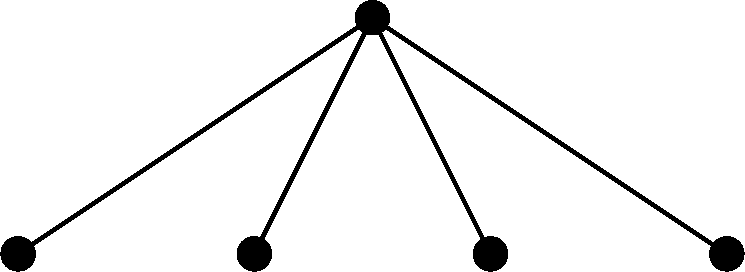
\includegraphics[height=1.2cm]{Pictures/Star_legs_4.pdf}
\end{center}
\end{ex}


\begin{ex}
 Let $R=K[x_1,\dots, x_n]$. Then the set of all monomials in $R$ equipped with the divisibility relation, that is,  the relation $\bx^\ba \mid \bx^\bb$ gives a partial order. This is because the statement $\bx^\ba \mid \bx^\bb$ translates into comparing the vectors of exponents in $\N^n$ by $\ba\leq \bb$ where the inequality is understood componentwise, that is, $a_i\leq b_i$ for $1\leq i\leq d$.  
\end{ex}

\begin{tcolorbox}
\begin{defn}\label{def: divisibility}
 Let $R=K[x_1,\dots, x_n]$, $I$ a homogeneous ideal of $R$ and $S=R/I$. Let $\M_S$ denote the set of monomials in $S$ and define for $f,g\in\M_S$ that $f$ divides $g$, denoted $f\mid g$, if  there exists $h \in\M_S$ such that $fh=g$.
 \end{defn}
 \end{tcolorbox}
 
 \begin{ex}\label{ex: x^2-y^2}
For divisibility  in quotient rings it is important to be aware that a monomial can be written in different ways. For example in $S=K[x,y]/(x^2-y^2)$ we have $x^2+I=y^2+I$. So  $x^2+I$ divides $y^3+I$ according to \Cref{def: divisibility} because 
\[
(x^2+I)(y+I)=(y^2+I)(y+I)=y^3+I.
\]
 \end{ex}

\begin{tcolorbox}[reset]
\begin{exer}\label{ex:poset M_S}
Show that divisibility in $\M_S$ is an order relation, so $\M_S$ is a poset. 
\end{exer}
\end{tcolorbox}


\begin{ex}\label{ex:diagram}
Below is the Hasse graph of $\M_S$ for
\[
S=K[x_1,x_2]/I \quad \text{ and } I=(x_1x_2-x_2^2, x_1^4,x_1^3x_2, x_1^2x_2^2, x_1^3x_2, x_1^4).
\]
\begin{center}
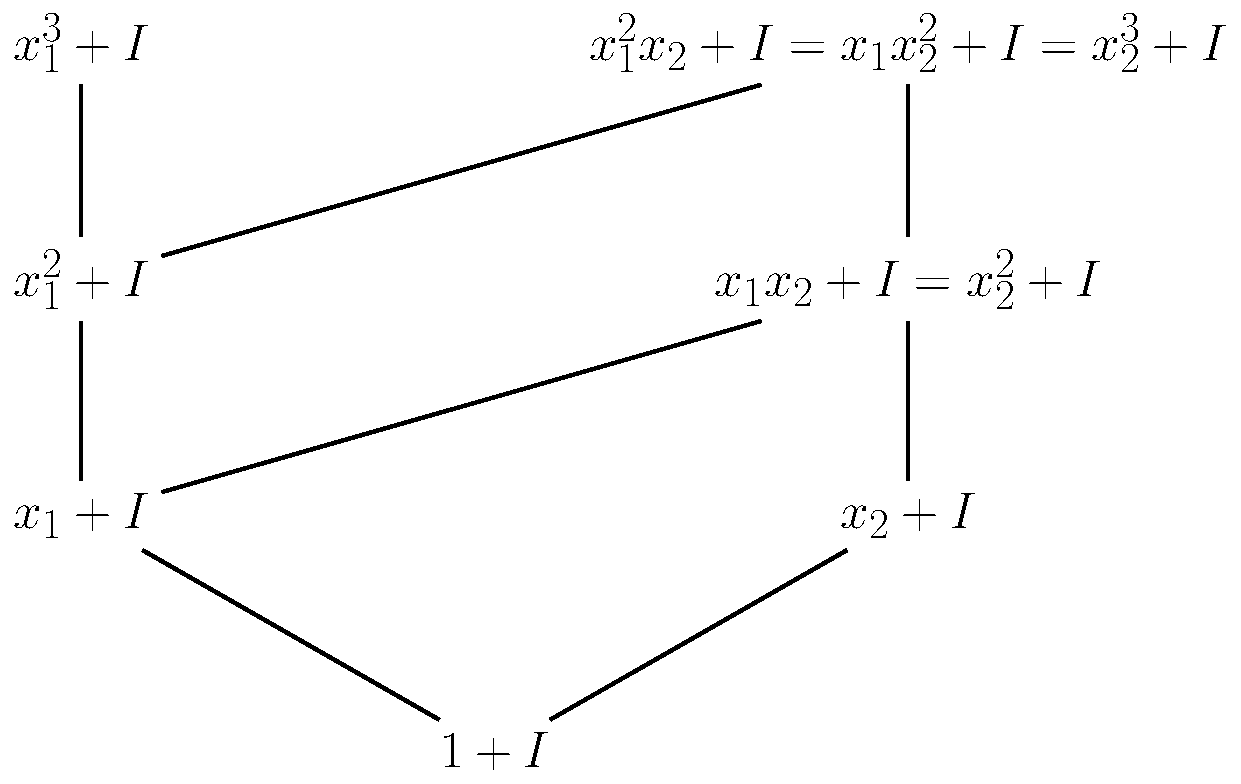
\includegraphics[width=0.43 \textwidth]{Pictures/glue_example.pdf}
\end{center}
\end{ex}

\begin{tcolorbox}[reset]
\begin{exer}
Draw the Hasse graph for the poset of monomials in \Cref{ex: x^2-y^2}.
\end{exer}
\end{tcolorbox}


\begin{ex}
The {\em box poset} $\M(d_1, \ldots, d_n)$ is the poset of monomials in $S=\frac{K[x_1,\ldots, x_n]}{(x_1^{d_1}, \ldots, x_n^{d_n})}$. This can be described in an alternative way as
\[
\M(d_1, \ldots, d_n)=\{\ba \in \N^n \mid 0\leq a_i<d_i \text{ for all } 1\leq i\leq n\}
\]
with the partial order given by componentwise inequality $\ba\leq \bb $ if $a_i\leq b_i$  for all  $1\leq i\leq n$.
\smallskip
\begin{center}
	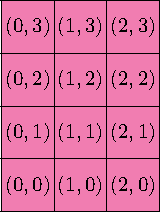
\includegraphics[height=3cm]{Pictures/2D_3_4.pdf}
	\qquad 
	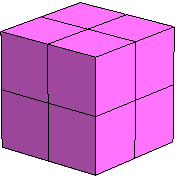
\includegraphics[height=3cm]{Pictures/3D_cube.pdf}
	\qquad 
	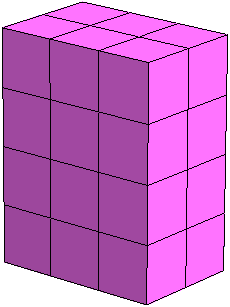
\includegraphics[height=3cm]{Pictures/3D_2_3_4.pdf}
\end{center}
\end{ex}


\begin{tcolorbox}[reset]
\begin{exer} Two different rings can have the same poset of monomials. Show that the posets of monomials $\M_S$ for $S=\frac{K[x_1,x_2,x_3]}{(x_1^{2}, x_2^2, x_3^{3})}$ and $\M_T$ for $T=\frac{K[x_1,x_2,x_3]}{(x_2^{2}, x_1x_3, x_1^2-x_3^{2})}$ have the same Hasse graph.
\end{exer}
\end{tcolorbox}


\begin{tcolorbox}
\begin{defn}
A poset $\P$ is {\bf ranked} if there is a function $r : \P \to \N$ called a {\em rank function} for which the following conditions hold:
\begin{itemize}
\item  There is a minimum element $x \in \P$ such that $r(x) = 0$.
\item If  $b$ covers $a$ in $\P$ then $r(b)=r(a)+1$.
\end{itemize}
For $d\in \N$, the $d$-th {\bf level} of $\P$ is $\P_d =\{x\in \P \mid r(x)=d\}$.
\end{defn}
\end{tcolorbox}

\begin{ex}
The posets of monomials discussed above are ranked. The rank function is given by taking the rank of a monomial to be its degree.
\end{ex}

\section{Macaulay Posets and Macaulay Rings} \label{s: 2}

\subsection{Macaulay Posets}
In this section we take a poset with its partial order, add  a {\em total} order on it, and study how it interacts with the partial order. If they interact well, we will say the poset is Macaulay.

\begin{tcolorbox}
\begin{defn}
For a subset $A$ of a poset $\P$ we define the {\bf upper shadow} of $A$ as
\[
\uSdw_\P A=\{b\in P : \text{there is an } a\in A \text{ such that } b \text{ covers } a\}
\]
and the {\bf lower shadow} of $A$ as
\[
\dSdw_\P A =\{b\in P :  \text{there is an } a\in A \text{ such that }  a \text{ covers } b\}.
\]
\end{defn}
\end{tcolorbox}

\begin{ex}
In the figure below on the left the set $A=\{xy,x^2\}$ is shown in pink and its lower shadow $\dSdw A=\{x,y\}$ is shown in green.  On the right  the set $A=\{xy,y^2\}$ is shown in pink and its upper shadow $\uSdw A=\{x^2y,xy^2,y^3\}$ is shown in green.
\begin{center}
	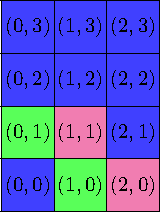
\includegraphics[height=4cm]{Pictures/2D_lower_shadow_set.pdf}
	\qquad 
	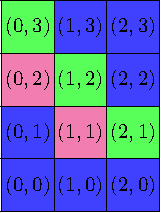
\includegraphics[height=4cm]{Pictures/2D_upper_shadow_set.pdf}
\end{center}
\end{ex}




\begin{ex}\label{ex: lex}
Let $\bx^\ba ,\bx^\bb$ be monomials in $R=K[x_1,\ldots,x_n]$. The inequality $\bx^\ba <_{\lex} \bx^\bb$ holds with respect to the {\em lexicographic order} (for short ex) if  the leftmost nonzero entry of $\ba-\bb$ is negative. This is a total order on $\M_R$. 

If $S=R/I$ is a quotient ring where $I$ is a {\em monomial ideal} then the lexicographic order is also defined on $\M_S$ in the same way: $\bx^\ba +I <_{\lex} \bx^\bb +I $ if $\bx^\ba <_{\lex} \bx^\bb$ in $R$.
\end{ex}



\begin{tcolorbox}
\begin{defn}
The {\bf initial segment} of size $q$ in the $d$-th level $\P_d$ of a ranked  poset $\P$ with an additional total order $\O$ is 
\[
\Seg_d q= \{ \text{the largest } q \text{ elements with respect to } \O  \text{ in } \P_d \}.
\]
\end{defn}
\end{tcolorbox}
\begin{ex}
The monomials of degree 2 in $K[x,y,z]$ are ordered with respect to the lexicographic order by
$x^2>xy>xz>y^2>yz>z^2$. Thus we have $\Seg_2 4=\{x^2, xy, xz, y^2\}$.
\end{ex}


%\begin{figure}
%\begin{center}
%	\animategraphics[loop,autoplay, height=5cm]{1.5}{2D_6_6_lex_}{0}{36}
%	\qquad
	%\animategraphics[loop,autoplay,height=5cm]{1.5}{5_5_5_Lex_}{1}{125}
%\end{center}
%\caption{The lexicographic order -- animation plays in Adobe Reader}
%\label{fig: lex}
%\end{figure}


\begin{tcolorbox}
\begin{defn}
A poset $\P$ with an additional order $<$ is called a {\bf Macaulay poset} if the following hold for any subset $A\subset \P_d$ 
\begin{enumerate}
\item {\em Initial segments have the smallest upper shadows}: 
\[
\left | \uSdw_\P\Seg_d |A|  \right | \leq  |\uSdw_\P(A)|;
\]
\item {\em The upper shadow of an initial segment is an initial segment}
\[
 \uSdw_\P  \Seg_d |A| =\Seg_{d-1} |\uSdw_\P(A)|.
\]
\end{enumerate}
\end{defn}
\end{tcolorbox}

\subsection{Macaulay Rings}

Before we talk about Macaulay rings we need to talk about a bit of book-keeping that has to do with monomials.

\begin{tcolorbox}
\begin{defn}
We say that a homogeneous quotient ring $S=R/I$ is {\bf level linearly independent} if for each degree $d$ the set of distinct monomials of degree $d$ in $R$ is linearly independnt over $K$, that is,  if  we have for some pairwise distinct monomials $\bm_1+I,\ldots, \bm_t+I\in S$ and  for some $k_1,\ldots, k_t\in K$ that
\[
k_1\bm_1 +\cdots+k_t \bm_t \in I 
\]
then we must have $k_1=\cdots =k_n=0$.
\end{defn}
\end{tcolorbox}

\begin{tcolorbox}[reset]
\begin{exer}
\begin{enumerate}
\item Prove that if $I$ is a monomial ideal, $S=R/I$ is level linearly independent.
\item Prove that if $I$ is generated by monomials and binomials, that is,  $I=(\bb_1, \ldots, \bb_s)$ with $\bb_i=\bm_i-\bm'_i$ for some $\bm_i,\bm'_i$ monomials in $R$,  then $S=R/I$ is level linearly independent.
\end{enumerate}
\end{exer}
\end{tcolorbox}


In the context of level linearly independent rings it makes sense to count the monomials in each degree.
\begin{tcolorbox}
\begin{defn}
The {\bf Hilbert function} of a level linearly independent homogeneous quotient ring $S=R/I$ is the function
\[
H_S:\N\to \N, \quad H_S(d)=\# \text{ of distinct monomials of degree } d \text{ in } S.
\]
The {\em Hilbert series} of $S$ is the formal sum $HS_S(t)=\sum_{d\geq 0} H_S(d)t^d$.
\end{defn}
\end{tcolorbox}

\begin{ex}
The ring $S$ in \Cref{ex:diagram} has Hilbert function 
\[
H_S(d)=\begin{cases}
1 & \text{ if } d=0\\
2 & \text{ if } 1\leq d\leq 3\\
0 & \text{ if } 4\leq d.
\end{cases}
\]
\end{ex}

\begin{tcolorbox}[reset]
\begin{exer}
Find the Hilbert series of the box ring $S=\frac{K[x_1,\ldots, x_n]}{(x_1^{d_1}, \ldots, x_n^{d_n})}$. {\em Hint:} \Cref{ex: tensor product} may help. Start with $n=1$ and $n=2$ to ease into this.
\end{exer}
\end{tcolorbox}

Now we are ready to translate the notion of Macaulay posets to rings. Like before we will consider a total order $\leq$ on the set of monomials $\M_S$ of a ring $S$. Such an order is a {\em monomial order} provided it satisfies
\[
\bm_1\leq \bm_2 \text{ implies } \bm_1 \bm'\leq \bm_2\bm' \text{ for any monomial } \bm'.
\]

\begin{tcolorbox}[reset]
\begin{exer}
The lexicographic order in \Cref{ex: lex} is a monomial order.
\end{exer}
\end{tcolorbox}

\begin{tcolorbox}
\begin{defn}
A homogeneous ring $S=R/I$ with monomial poset $\M_S$ endowed with a total order $\O$ is a {\bf Macaulay ring} provided that for $\bm+I$ a monomial in $S$
\[
d\geq 0, 1\leq i\leq n \text{ and } \bm+I\in \Seg_d H_S(d) \text{ imply } x_i\bm +I \in  \Seg_d H_S(d).
\]
\end{defn}
Equivalently, $S$ is a {\em Macaulay ring} provided the following set is an ideal
\[
\O(I)=\bigoplus_{d\geq 0} \Span_K \Seg_d H_S(d).
\]
\end{tcolorbox}

The most important Macaulay rings are the following:
\begin{thm}
\begin{enumerate}
\item (Macaulay's Theorem) The polynomial ring $R=K[x_1,\ldots, x_n]$ with the  lexicographic total order is Macaulay.
\item (Clements-Lindstr\"om Theorem) The box ring    $S=\frac{K[x_1,\ldots, x_n]}{(x_1^{d_1}, \ldots, x_n^{d_n})}$ is Macaulay with respect to the lexicographic order  if $d_1\leq d_2\leq \ldots \leq d_n$.
\end{enumerate}
\end{thm}

Also, there is a perfect correspondence between Macaulay rings and Macaulay posets in the following form: a homogeneous ring $S$ is Macaulay with respect to a total order  if and only if $\M_S$ is a Macaulay poset with respect to the same total order; see \cite[Theorem 2.6.3]{Nik}.


\section{Constructing new rings and posets}\label{s:3}
 In this section we describe the problems that we will be working on. Generally speaking these problems have to do with combining simple rings to make more complicated rings. Then we will ask: if the simple rings are Macaulay, can we deduce that the more complicated ones are?

A simple way to combine two posets is to take their cartesian product. This corresponds to a tensor product of rings when we have level linear independence.
\begin{tcolorbox}
\begin{defn}
Suppose that we have posets $\P_i$ with $1\leq i\leq t$. Their {\bf cartesian product} is the set
\[
\P_1\times \P_2 \times \cdots  \times \P_t=\{(p_1,\ldots, p_s): p_i\in \P_i\}
\]
with the partial order $(p_1,\ldots, p_s)\leq (p'_1,\ldots, p'_s)$ if and only if $p_i\leq p'_i$ for $1\leq i\leq t$.
\end{defn}
\end{tcolorbox}

\begin{tcolorbox}
\begin{defn}
Suppose that we have rings $S_i = R_i/I_i$ for some homogeneous ideal $I_i$ of $R_i = K[x_{i,1}, \ldots, x_{i,n_i} ]$. Their  {\bf tensor product} over $K$ is the ring
\[
S_1\otimes_K \cdots \otimes_K S_t = K[x_{1,1},\ldots,x_{1,n_1},\ldots,x_{t,1},\ldots,x_{t,n_t}]/ (I_1 +I_2 +\cdots +I_t).
\]
where $I_1 +I_2 +\cdots +I_t=\{f_1+f_2+\cdots+f_t: f_i\in I_i \text{ for } 1\leq i\leq t\}$.
\end{defn}
\end{tcolorbox}
The correspondence between these notions is given by: if $S=S_1\otimes_K \cdots \otimes_K S_t $ then $\M_S=\M_{S_1}\times \cdots \times \M_{S_t}$. 

\begin{ex}\label{ex: tensor product}
If for $1\leq i\leq n$ we set $S_i=K[x_i]/(x_i^{d_i})$ then $S=S_1\otimes_K S_2\otimes_K \cdots \otimes_K S_n=K[x_1,\ldots, x_n]/(x_1^{d_1},\ldots, x_n^{d_n})$. This gives a decomposition of the box ring into rings $S_i$ for which the posets $\M_{S_i}$ are chains.
\end{ex}



\begin{tcolorbox}[reset]
\begin{oprobl}\label{oprobl 1}
\begin{enumerate}
\item If $\P$ is a Macaulay poset,  is $\P\times \P\times \cdots \times \P$ a Macaulay poset?
\item If $S$ is a Macaulay ring, is  $S\otimes_K S\otimes_K \cdots \otimes_K S$  a Macaulay ring?
\item If $\P_1, \ldots, \P_t$ are Macaulay posets,  is $\P_1\times \P_2\times \cdots \times \P_t$ a Macaulay poset?
\item If $S_1, \ldots, S_t$ are Macaulay rings,  is $S_1\otimes_K S_2\otimes_K \cdots \otimes_K S_t$ a Macaulay ring?
\end{enumerate}
\end{oprobl}
\end{tcolorbox}

Some particular cases of \Cref{oprobl 1} are known: the answer to (1) is known only for lexicographic order; see \cite{uwsuper}. A special case of (2) can be found in \cite[Theorem 4.1]{Mermin}. See also Theorem 10 in \cite{survey}  for a partial answer.

There are several other ways of combining rings.

\begin{tcolorbox}
\begin{defn}
Suppose that for $1\leq i\leq t$ we have posets $\P_i$ with unique least element $\ell_i$. Their {\bf wedge product} is the set
\[
\P_1\vee \P_2 \vee \cdots \vee  \P_t=\left(\bigsqcup_{i=1}^t P_i \right)/ (\ell_1=\ell_2=\cdots  =\ell_t),
\]
(meaning that we take the disjoint union of the sets $\P_i$ in which we identify all the $\ell_i$ into one element)
with the partial order $a\leq b$ if and only if $a\leq b$ in $\P_i$ for some $i$.
\end{defn}
\end{tcolorbox}

\begin{ex}\label{ex: spider poset}
A {\em spider} poset with legs of length $d_1,\ldots, d_t$ is the wedge product of $t$ path posets of lengths $d_1, d_2, \ldots, d_t$ respectively. Here are some Hasse graphs of spider posets:
\begin{center}

\includegraphics[height=1.95cm]{Pictures/Spider_legs_1_length_2.pdf}
\qquad 
\rotatebox[origin=c]{180}{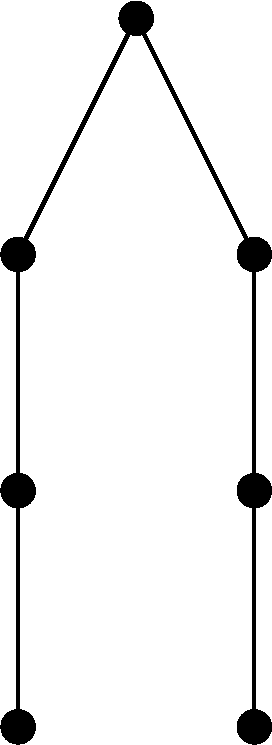
\includegraphics[height=1.95cm]{Pictures/Spider_legs_2_length_3.pdf}}
\qquad 
\rotatebox[origin=c]{180}{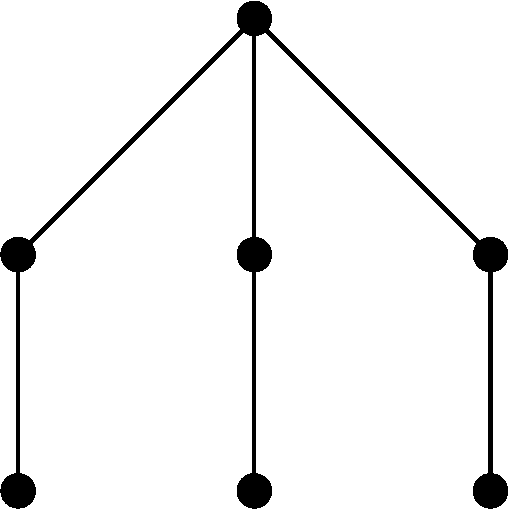
\includegraphics[height=1.95cm]{Pictures/Spider_legs_3_length_2.pdf}}
\end{center}
\end{ex}

\begin{tcolorbox}
\begin{defn}
Suppose that we have rings $S = R/I$  and $T=R'/J$ for some homogeneous ideals $I$ of $R = K[x_1,\ldots, x_n]$ and $J$ of $R'=K[y_1, \ldots, y_m]$. Their  {\bf fiber product} over $K$ is the ring
\[
S\times_K T= K[x_1,\ldots, x_n, y_1, \ldots, y_m]/ (I +J + (x_iy_j: 1\leq i\leq n, 1\leq j\leq m)).
\]
\end{defn}
\end{tcolorbox}

\begin{tcolorbox}[reset]
\begin{exer}
Prove that $\M_{S\times_K T}=\M_S\vee \M_T$.
\end{exer}
\end{tcolorbox}

\begin{tcolorbox}[reset]
\begin{oprobl}\label{oprobl 2}
\begin{enumerate}
\item If $\P$ is a Macaulay poset,  is $\P\vee \P\vee \cdots \vee \P$ a Macaulay poset?
\item If $S$ is a Macaulay ring, is  $S\times_K S\times_K \cdots \times_K S$  a Macaulay ring?
\item If $\P_1, \ldots, \P_t$ are Macaulay posets,  is $\P_1\vee \P_2\vee \cdots \vee \P_t$ a Macaulay poset?
\item If $S_1, \ldots, S_t$ are Macaulay rings,  is $S_1\times_K S_2\times_K \cdots \times_K S_t$ a Macaulay ring?
\end{enumerate}
\end{oprobl}
\end{tcolorbox}

With respect to \Cref{oprobl 2} spider posets (see \Cref{ex: spider poset}) are the only examples of wedge products known to be Macaulay in the literature. This is because the wedge product construction was previously only used on an ad-hoc basis in the literature. Another direction that one can take is to combine several of the operations discussed above. For example, the cartesian product of spiders with the same number of legs is  shown to be Macaulay in \cite{Bez2}. The case of a cartesian product of spiders with different numbers of legs is an open conjecture therein, which seems rather difficult.

The wedge construction identified the least elements of some posets. By contrast, the next diamond construction identifies both the least and largest elements.


\begin{tcolorbox}
\begin{defn}
Suppose that for $1\leq i\leq t$ we have posets $\P_i$ with unique least element $\ell_i$ and unique largest element $L_i$. Their {\bf diamond product} is the set
\[
\P_1\di \P_2 \di \cdots \di  \P_t=\left(\bigsqcup_{i=1}^t P_i \right)// (\ell_1=\ell_2=\cdots \cdots \ell_t, L_1=L_2=\cdots=L_t ),
\]
(meaning that we take the disjoint union of the sets $\P_i$ in which we identify all the $\ell_i$ into one element and all the $L_i$ elements into one element)
with the partial order $a\leq b$ if and only if $a\leq b$ in $\P_i$ for some $i$.
\end{defn}
\end{tcolorbox}

\begin{ex}\label{ex: diamond}\label{ex: tori diamond}
Here are some Hasse graphs of diamond products of path posets:
\begin{center}
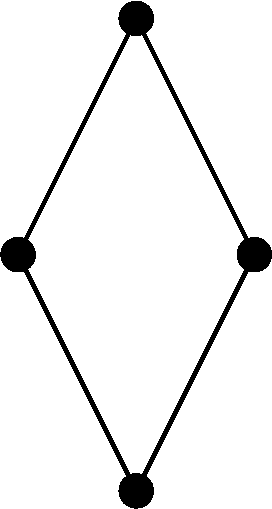
\includegraphics[height=2cm]{Pictures/Torus_4.pdf}
\quad 
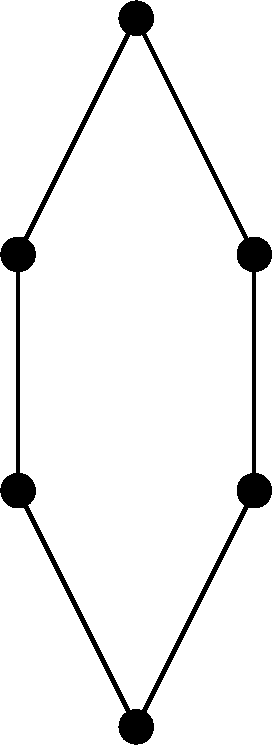
\includegraphics[height=2cm]{Pictures/Torus_6.pdf}
\quad
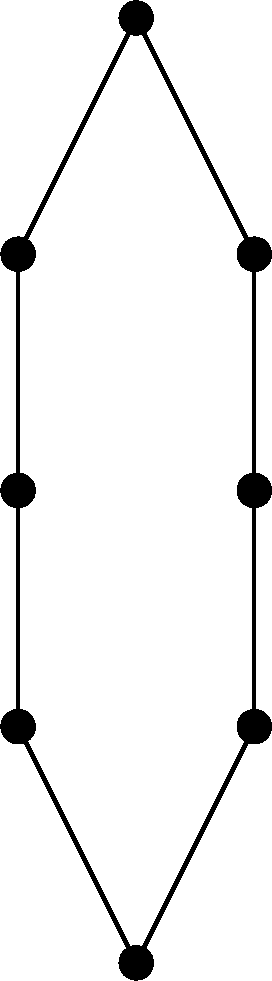
\includegraphics[height=2cm]{Pictures/Torus_8.pdf}
\quad
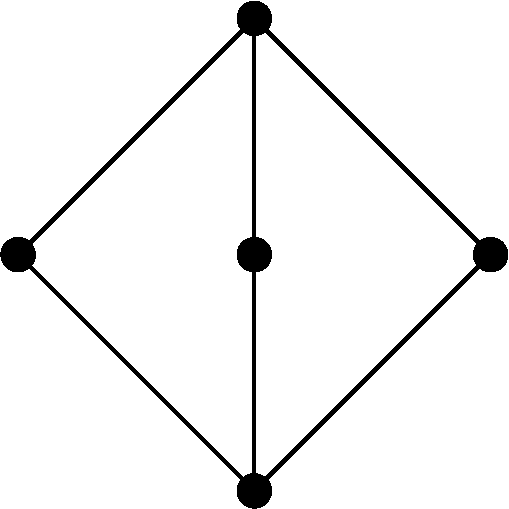
\includegraphics[height=2cm]{Pictures/Diamond.pdf}
\end{center}
Diamond products of two path posets of the same length such as the leftmost three posets above are called {\em discrete tori}. The rightmost poset above is called a {\em diamond poset}.
\end{ex}

In the previuous pictures we have taken diamond products of path posets of the same length. This ensures that the result is a ranked poset.
\begin{tcolorbox}[reset]
\begin{exer}
Prove that for ranked posets $\P_i$ with the maximum rank of elements in $\P_i$ equal to $r_i$ the poset $P_1\di \P_2 \di \cdots \di  \P_t$ is ranked if and only if $r_1=r_2=\cdots=r_t$.
\end{exer}
\end{tcolorbox}


\begin{tcolorbox}
\begin{defn}
Suppose that we have rings $S = R/I$  and $T=R'/J$ for some homogeneous ideals $I$ of $R = K[x_1,\ldots, x_n]$ and $J$ of $R'=K[y_1, \ldots, y_m]$ such that $\M_S$ and $\M_T$ have unique maximal elements $\bm_S$ and $\bm_T$ respectively, called {\em socle elements}, (Such rings $S$ and $T$ are called Gorenstein). Their  {\bf connected sum} over $K$ is the ring
\[
S\#_K T= K[x_1,\ldots, x_n, y_1, \ldots, y_m]/ (I +J + (x_iy_j: 1\leq i\leq n, 1\leq j\leq m)+(\bm_S-\bm_T)).
\]
\end{defn}
\end{tcolorbox}


\begin{tcolorbox}[reset]
\begin{oprobl}\label{oprobl 3}
\begin{enumerate}
\item If $\P$ is a Macaulay poset,  is $\P\di \P\di \cdots \di \P$ a Macaulay poset?
\item If $S$ is a Macaulay ring, is  $S\#_K S\#_K \cdots \#_K S$  a Macaulay ring?
\item If $\P_1, \ldots, \P_t$ are Macaulay posets,  is $\P_1\di \P_2\di \cdots \di \P_t$ a Macaulay poset?
\item If $S_1, \ldots, S_t$ are Macaulay rings,  is $S_1\#_K S_2\#_K \cdots \#_K S_t$ a Macaulay ring?
\end{enumerate}
\end{oprobl}
\end{tcolorbox}

As with the wedge product construction, the diamond product is formalized here for the first time. Thus \Cref{oprobl 3} is only known for products of discrete tori and for the diamond poset (see \Cref{ex: tori diamond}). 
The next interesting case is the diamond product of 3 paths of the same length $>3$. We suspect this example may be Macaulay but others may not be. The case of cartesian product of such posets is extremely interesting, but will be significantly more challenging to decide whether it is Macaulay.

More generally, one can construct fiber product rings and posets and connected sum rings and posets over rings or posets other than $K$, meaning that instead of identifying the least element and the largest element we identify more elements  given by a common subposet $\P_C$. 

\begin{tcolorbox}
\begin{defn}\label{def: fiber prod poset}
Suppose there are inclusions of posets $\iota_A:\P_C\hookrightarrow \P_A$ and $\iota_B:\P_C\hookrightarrow\P_B$. The the {\em fiber product poset} is the set
\[
\P_A\times_{\P_C} \P_B = \P_C \sqcup \left \{ a : a\in \P_A\setminus \iota_A(\P_C)\right \} \sqcup \left \{ b : b \in \P_B\setminus \iota_B(\P_C)\right \}
\]
with order relation 
\begin{itemize}
\item $a\geq c$ iff $a\geq \iota_A(c)$ for $a\in \P_A\setminus \iota_A(\P_C)$ and $c\in \P_C$ and
\item $b\geq c$ iff $b\geq \iota_B(c)$ for $b\in \P_B\setminus \iota_B(\P_C)$ and $c\in \P_C$.
\end{itemize}
\end{defn}
\end{tcolorbox}

\begin{ex}
If $\P_A$ and $\P_B$ are both path posets of length $3$ and $\P_C$ is a sub-path of length 2 containing the least element of  $\P_A$ and $\P_B$, 
the resulting fiber product is
\begin{center}
	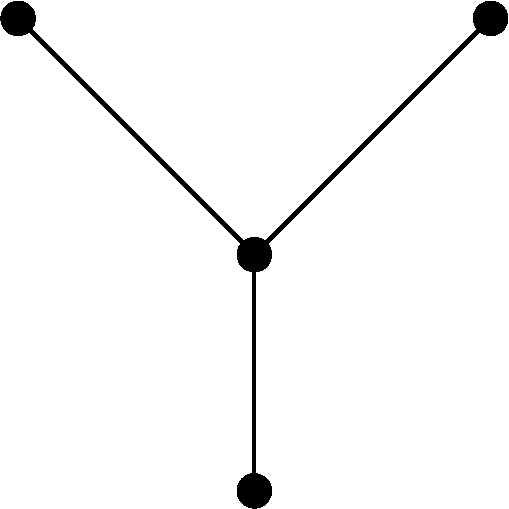
\includegraphics[height=1.95cm]{Pictures/fiber_product_hasse.pdf}
\end{center}
\end{ex}

%The {\em dual} $\P^*$ of a poset $\P$ is the poset on the same elements as $\P$, but with the order reversed, that is, if $a\leq b$ in $\P$ then $b\leq a$ in $\P^*$. A poset $\P$ is {\em self-dual} if $\P$ and $\P^*$ have the same Hasse graph. For example, paths and box posets are self-dual and so are the posets in \Cref{ex: diamond}.
%
%\begin{tcolorbox}
%\begin{defn}
%Suppose that $\P_A, \P_B$ are self-dual posets and that there are  inclusions of posets $\iota_A:\P_C\hookrightarrow \P_A$,  $\iota_B:\P_C\hookrightarrow\P_B$, $\iota'_A:\P_C^*\hookrightarrow \P_A$,  $\iota'_B:\P_C^*\hookrightarrow\P_B$. The the {\em connected sum poset} is 
%\[
%\P_A\times_{\P_C} \P_B = \P_C \sqcup \P_C^* \left \{ a : a\in \P_A\setminus \P_C\right \} \sqcup \left \{ b : b \in \P_B\setminus \P_C\right \}
%\]
%with order relation 
%\begin{itemize}
%\item $a\geq c$ iff $a\geq \iota_A(c)$ for $a\in \P_A\setminus \P_C$ and $c\in \P_C$ and
%\item $b\geq c$ iff $b\geq \iota_B(c)$ for $b\in \P_B\setminus \P_C$ and $c\in \P_C$.
%\end{itemize}
%\end{defn}
%\end{tcolorbox}
%

This notion corresponds to an operation on rings defined as follows.

\begin{tcolorbox}
\begin{defn}\label{def: fiber product rings}
Suppose we have surjective ring maps $\pi_A:A\hookrightarrow C$ and $\pi_B:B\to C$. The the {\em fiber product} of $A$ and $B$ over $C$ is the ring
\[
A\times_C B= \{(a,b): a\in A, b\in B, \pi_A(a)=\pi_B(b)\}.
\]
\end{defn}
\end{tcolorbox}

In \Cref{def: fiber prod poset} we identify a copy of $\P_C$ in each of $\P_A$ and $\P_B$. We can also identify two copies of $\P_C$ one at the ``bottom" and one at the ``top" of each of two posets. To be able to do this $\P_A$ and $\P_B$ must be self-dual, that is, their Hasse graphs must remain unchanged when flipped upside-down. The resulting poset is called a {\em connected sum}. Both connected sums and fiber products originate in algebraic topology, a study of shapes and their deformations.

Rather than giving a general definition, I will give an example that illustrates how the procedure of taking connected sum works starting from two box rings.


\begin{ex}\label{ex: connected sum}
We start with $\P_A=\P_B$ being $3\times 2$ box posets and $\P_C$ being a length $2$ chain (which is also a $1\times 2$ box poset). The copy of $\P_C$ at the ``bottom" of $\P_A$ and $\P_B$ is drawn in blue and the one at the ``top" in red. After identifying them we get the poset on the right.
\begin{center}
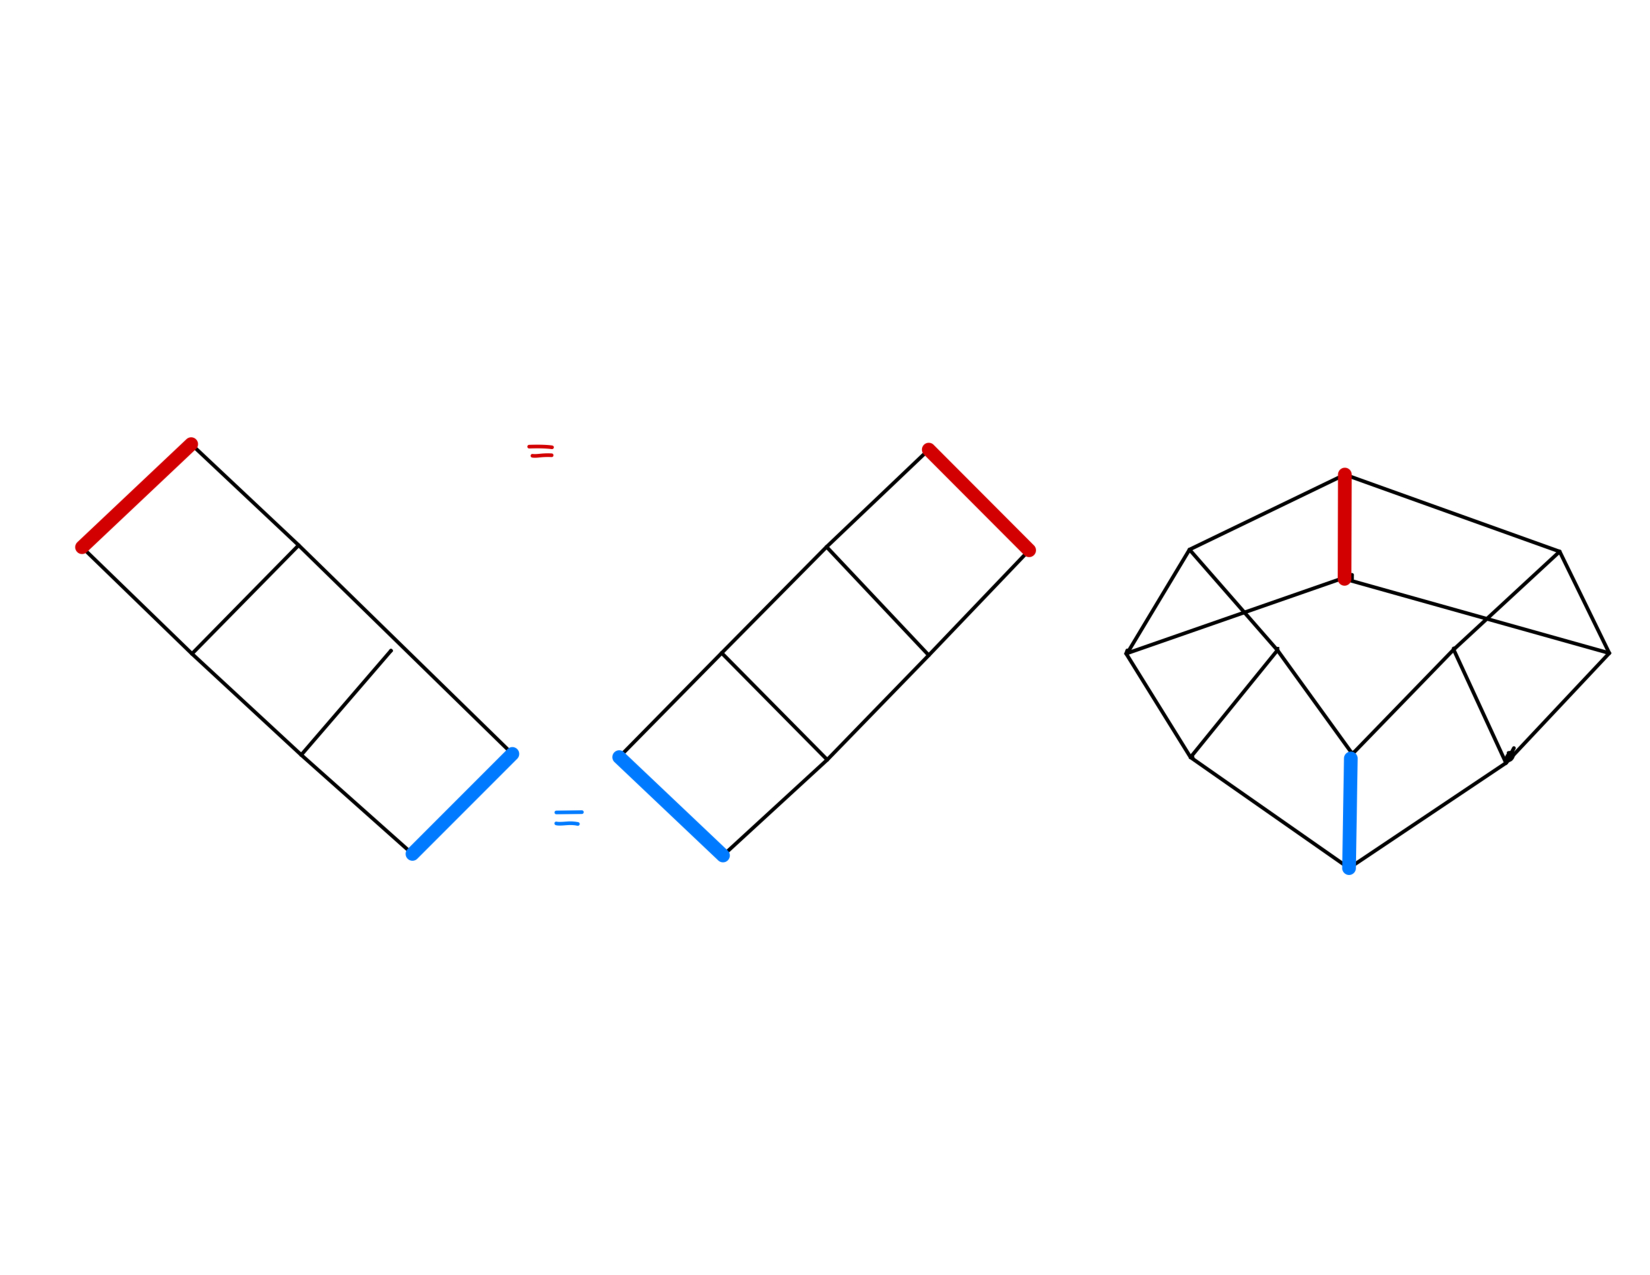
\includegraphics[width=\textwidth]{Pictures/ConnectedSum.pdf}
\end{center}
\end{ex}

Now we define the connected sum of two box rings algebraically.
\begin{tcolorbox}
\begin{defn}\label{def: connected sum rings}
Define an operation on monomials by 
\[
\bx^{\mathbf{d}} \circ \bx^\be= \begin{cases}
\bx^{\be-\mathbf{d}}=x_1^{e_1-d_1}\cdots x_n^{e_n-d_n} & \text{ if } \mathbf{d}\leq \be\\
0 & \text{ otherwise}
\end{cases}
\]
and extend it to polynomials linearly, that is, 
\[
(\sum_{i=1}^s \bm_i)\circ (\sum_{j=1}^t \bm'_j)=\sum_{i=1}^s\sum_{j=1}^t  \bm_i\circ \bm'_j.
\]
Fix $\ba, \bb\in \N^n$ to be vectors that have the same sum and let $\bx^\bc=\gcd(\bx^\ba, \bx^\bb)$. If\footnote[2]{This requirement ensures that the two copies of $\M_C$ at the top and botton of $\M_A, \M_B$ are disjoint.} $\bx^\ba \nmid (\bx^\bc)^2$ and $\bx^\bb \nmid (\bx^\bc)^2$, then the quotient ring
 \[
 R/(f\in R : f\circ(\bx^\ba+\bx^\bb)=0)
 \]
 is the {\bf connected sum} of  box rings $A=R/(x_1^{a_1+1},\ldots, x_n^{a_n+1})$ and $B=R/(x_1^{b_1+1},\ldots, x_n^{b_n+1})$ over  $C=R/(x_1^{c_1+1},\ldots, x_n^{c_n+1})$, denoted $A\#_C B$.
 \end{defn} 
\end{tcolorbox}

\begin{ex}
We recreate \Cref{ex: connected sum} with rings by setting $\ba=(3,1,0)$, $\bb=(0,1,3)$ and $\bc=(0,1,0)$. Then the construction above yields 
 \[
 A\#_C B=\frac{K[x_1,x_2,x_3]}{(x_1x_3, x_2^2, x_1^3-x_3^3)}.
 \]
\end{ex}

\begin{tcolorbox}[reset]
\begin{exer}
Check that the example above matches \Cref{def: connected sum rings} and check that the poset of monomials of this ring mathches \Cref{ex: connected sum}.
\end{exer}
\end{tcolorbox}

Now we can ask questions regarding the ability of these constructions to produce Macaulay rings and posets.

\begin{tcolorbox}[reset]
\begin{oprobl}\label{oprobl 4}
\begin{enumerate}
\item If $\P_A, \P_B,\P_C$ are Macaulay is the fiber product poset in \Cref{def: fiber prod poset} Macaulay?
\item If $A, B, C$ are Macaulay rings is the fiber product ring $A\times_C B$  in \Cref{def: fiber product rings} Macaulay?
\item  Is the connected sum poset from \Cref{ex: connected sum} Macaulay?
\item Is the connected sum ring from \Cref{def: connected sum rings} Macaulay? 
\end{enumerate}
\end{oprobl}
\end{tcolorbox}

\Cref{oprobl 4} is largely unexplored except for the particular case of fiber products and connected sums over $K$, which are \Cref{oprobl 2} and \Cref{oprobl 3} respectively. Since this is a new area we reconned to start by studying the poset in \Cref{ex: connected sum} in as much detail as possible.

For all of the open problems  stated in this document one should try first to work out as many examples as possible. We expect that some examples you will find will be Macaulay and others will not be. Then we can try to formulate conditions  under which these operations lead to Macaulay results. The main difficulty is that the total order $\O$ in the definition of Macaulay poset or ring is unspecified. This means you have the freedom to choose your order. One should probably try the lexicographic order first since this is often but not always known to work, but if it does not work you can try to make your own total orders to suit the example at hand. 
 

\vspace{1em}

\begin{thebibliography}{99}

\bibitem[BE]{Bez2} S.\,L\, Bezrukov and R.\, Els\"{a}sser, {\em The spider poset is Macaulay}
J. Combin. Theory Ser. A 90 (2000), no. 1, 1--26, available at \url{https://www.sciencedirect.com/science/article/pii/S0097316599929941}.

\bibitem[BL]{survey} S.\,L\, Bezrukov and U.\,Leck {\em Macaulay posets}, Electron. J. Combin. DS12 (2004), available at \url{https://www.combinatorics.org/files/Surveys/ds12/ds12v2-2005.pdf}.

\bibitem[BPS]{uwsuper} S.\,L\, Bezrukov, X.\,Portas, O.\,Serra, {\em A local-global principle for Macaulay posets} Order 16 (1999), no. 1, 57--76, available at  \url{http://cs2.uwsuper.edu/sb/Papers/lgp.pdf}.

\bibitem[CLO]{CLO}
D.\,Cox, J.\,Little, D.\,O'Shea, 
{\em Ideals, varieties, and algorithms. An introduction to computational algebraic geometry and commutative algebra}, Undergraduate Texts in Mathematics. Springer, Cham, 2015.

 \bibitem[M2]{M2}
D.\,Grayson and M\,Stillman,  {\em Macaulay2, a software system for research in algebraic geometry},
 available at \url{https://faculty.math.illinois.edu/Macaulay2/}.
 
 \bibitem[Kuz]{Nik}
N.\,Kuzmanovski,
{\em Macaulay posets and rings}, preprint (2023), available at \url{https://arxiv.org/pdf/2307.05094}.


 
 \bibitem[MP]{Mermin}J.\,Mermin and I.\,Peeva, {\em Lexifying ideals}, Math. Res. Lett.13 (2006), no.2-3, 409--422, available at \url{https://math.okstate.edu/people/mermin/papers/lexifying_ideals.pdf}.


%\bibitem[OEIS]{OEIS} 
%The On-Line Encyclopedia of Integer Sequences, \url{https://oeis.org}.

\end{thebibliography}


\end{document}

